\documentclass[a4paper]{article}
\usepackage{setspace}
\usepackage[T2A]{fontenc} %
\usepackage[utf8]{inputenc} % подключение русского языка
\usepackage[russian]{babel} %
\usepackage[14pt]{extsizes}
\usepackage{mathtools}
\usepackage{graphicx}
\usepackage{fancyhdr}
\usepackage{amssymb}
\usepackage{amsmath, amsfonts, amssymb, amsthm, mathtools}
\usepackage{tikz}

\usetikzlibrary{positioning}
\setstretch{1.3}

\newcommand{\mat}[1]{\begin{pmatrix} #1 \end{pmatrix}}
\renewcommand{\f}[2]{\frac{#1}{#2}}
\newcommand{\dspace}{\space\space}
\newcommand{\s}[2]{\sum\limits_{#1}^{#2}}
\newcommand{\sq}[1]{\left[ {#1} \right]}
\newcommand{\gath}[1]{\left[ \begin{array}{@{}l@{}} #1 \end{array} \right.}
\newcommand{\case}[1]{\begin{cases} #1 \end{cases}}
\newcommand{\ts}{\text{\space}}
\newcommand{\lm}[1]{\lim\limits_{#1}}

\newcommand{\lr}{\Leftrightarrow}
\renewcommand{\r}{\Rightarrow}
\newcommand{\rr}{\rightarrow}
\renewcommand{\geq}{\geqslant}
\renewcommand{\leq}{\leqslant}
\newcommand{\RR}{\mathbb{R}}
\newcommand{\CC}{\mathbb{C}}
\newcommand{\QQ}{\mathbb{Q}}
\newcommand{\ZZ}{\mathbb{Z}}
\newcommand{\VV}{\mathbb{V}}
\newcommand{\NN}{\mathbb{N}}

\DeclarePairedDelimiter\abs{\lvert}{\rvert} %
\makeatletter                               % \abs{}
\let\oldabs\abs                             %
\def\abs{\@ifstar{\oldabs}{\oldabs*}}       %

\begin{document}

\section*{Домашняя работа №5 (Математический анализ)}
{\large Емельянов Владимир, ПМИ гр №247}\\\\
\begin{enumerate}
    \item[\textbf{1.}]
    \begin{enumerate} 
        \item[(a)]Будем считать что пары целых - это координаты на плоскости. Чтобы построить биекцию, начнём отображать натуральные числа в эти координаты таким образом:\\
        $$1 \to (0, 0)$$
        $$2 \to (0, 1)$$
        $$3 \to (1, 1)$$
        $$\dots$$
        Продолжим идти в координатной плоскости "по спирали"\ts сопоставляя натуральные числа и пары целых:\\
        \[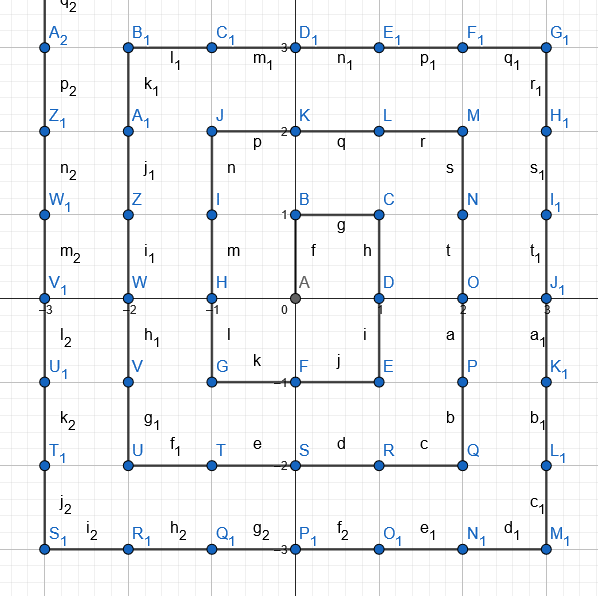
\includegraphics[width=0.4\textwidth]{image.png}\]
        Таким образом, мы отображаем все натуральные во все пары целых. \textbf{Это отображение является биекцией}
    
        \item[(b)]$A = [0;1],\ts B = [0;1)$\\
        Нам нужно "переселить" \ts $1$ из множества $A$, для этого отобразим элементы множества $ \{ \frac{1}{n} \mid n \in \NN \} \subset A$ из $A$ в $B$, такой функцией:
        $$f(\f{1}{n})=\f{1}{n+1} \text{, где } n \in \NN.$$
        То есть:
        $$A_0 \to B_0$$
        $$1 \to \f{1}{2}$$
        $$\f{1}{2} \to \f{1}{3}$$
        $$\dots$$
        $$\f{1}{n} \to \f{1}{n+1}$$
        Эта функция корректна, так как для каждого натурального $n$, элемент $\frac{1}{n+1} \in B $\\
        Теперь рассмотрим оставшуюся часть множества $ A $, а именно $[0;1] \setminus \{\frac{1}{n} \mid n \in \mathbb{N} \}$. Это множество, кроме точек вида $ \frac{1}{n} $, содержит такие элементы, как 0, и все иррациональные числа на отрезке $ [0;1] $.

        Для этих элементов мы можем построить биекцию напрямую:
        $$f(x) = x \quad \text{для всех} , x \in [0;1] \setminus \{ \frac{1}{n} \mid n \in \mathbb{N} \}$$
        Таким образом, мы построили биекцию между множествами $A = [0;1]$ и $B = [0;1)$, с помощью двух случаев.
    \end{enumerate}

    \item[\textbf{2.}]
    \begin{enumerate}
        \item[(a)] 
        $$a_n = \f{((-1)^n - 1)n^2 +n + 1}{n}$$
        $$\case{
            a_n = 1 + \f{1}{n} \text{ - если $n$ чётное}\\
            a_n = \f{-2n^2+n+1}{n} = -2n+1 + \f{1}{n} \text{ - если $n$ нечётное}
        }$$
        $$a_0 = 0, a_1 = \frac{3}{2}, a_2 = \frac{-14}{3}, a_3 = \frac{5}{4}, a_4 = \frac{-44}{5}, a_5 = \frac{7}{6}, a_6 = \frac{-90}{7},$$
        $$a_7 = \frac{9}{8}, a_8 = \frac{-152}{9}, a_9 = \frac{11}{10} $$
        Найдём $\overline{\lim}_{n \to \infty} a_n= \lim_{n \to \infty} M_n$
        $$M_1 = \frac{3}{2}, M_2 = \frac{5}{4}, M_3 = \frac{5}{4}, M_4 = \frac{7}{6}, M_5 = \frac{7}{6}, M_6 = \frac{9}{8},$$ 
        $$M_7 = \frac{9}{8}, M_8 = \frac{11}{10}, M_9 = \frac{11}{10} \r$$
        $$\r M_n = \f{n+1-n\%2+2}{n+1-n\%2+1} = \f{n-n\%2+3}{n-n\%2+2}$$
        $$\lim_{n \to \infty} M_n =\lim_{n \to \infty} \f{n-n\%2+3}{n-n\%2+2} = \lim_{n \to \infty}\f{1-\f{n\%2}{n}+\f{3}{n}}{1-\f{n\%2}{n}+\f{2}{n}} = \f{1-0+0}{1-0+0} = 1$$
        Найдём $\underline{\lim}_{n \to \infty} a_n= \lim_{n \to \infty} m_n$
        $$m_1 = \frac{-152}{9}, m_2 = \frac{-152}{9}, m_3 = \frac{-152}{9}, m_4 = \frac{-152}{9}, m_5 = \frac{-152}{9},$$ $$m_6 = \frac{-152}{9},
        m_7 = \frac{-152}{9}, m_8 = \frac{-152}{9}, m_9 = \frac{-152}{9} \r \lim_{n \to \infty} m_n = -\infty$$
        \textbf{Ответ: } $\lim_{n \to \infty} M_n = 1, \ts \lim_{n \to \infty} m_n = -\infty$
        
        \item[(b)]$$a_n = \f{n}{n+1}\cos\f{\pi n}{2}$$
        $$ a_1 = 0, a_2 = -\frac{2}{3}, a_3 = 0, a_4 = \frac{4}{5}, a_5 = 0, a_6 = -\frac{6}{7}, a_7 = \f{8}{9}$$
        Найдём $\overline{\lim}_{n \to \infty} a_n= \lim_{n \to \infty} M_n$:
        $$M_1 = \f{8}{9}, M_2 = \f{8}{9}, M_3 = \f{8}{9}, M_4 = \f{8}{9}, M_5 = \f{8}{9} \r $$
        $$\r M_n = max(a_n) \r \lim_{n \to \infty} M_n = 1$$
        Найдём $\underline{\lim}_{n \to \infty} a_n= \lim_{n \to \infty} m_n$:
        $$m_1 = -\f{6}{7}, m_2 = -\f{6}{7}, m_3 = -\f{6}{7}, m_4 = -\f{6}{7}, m_5 = -\f{6}{7} \r$$
        $$\r m_n = min(a_n) \r \lim_{n \to \infty} m_n = -1$$
        \textbf{Ответ: } $\lim_{n \to \infty} M_n = 1, \ts \lim_{n \to \infty} m_n = -1$

        \item[(c)]$$a_n = 1+2(-1)^{n+1} + 3(-1)^{\f{n(n-1)}{2}}$$
        {\small $$a_1 = 6, a_2 = -4, a_3 = 0, a_4 = 2, a_5 = 6, a_6 = -4, a_7 = 0, a_8 = 2$$}
        Найдём $\overline{\lim}_{n \to \infty} a_n= \lim_{n \to \infty} M_n$:
        $$M_1 = 6, M_2 = 6, M_3 = 6, \dots \r M_n = max(a_n) \r $$
        $$\lim_{n \to \infty} M_n = 6$$
        Найдём $\underline{\lim}_{n \to \infty} a_n= \lim_{n \to \infty} m_n$:
        $$m_1 = -4, m_2 = -4, m_3 = -4, \dots \r m_n = min(a_n) \r $$
        $$\lim_{n \to \infty} m_n = -4$$
        \textbf{Ответ: } $\lim\limits_{n \to \infty} M_n = 6, \ts \lim\limits_{n \to \infty} m_n = -4$
    \end{enumerate}

    \item[\textbf{3.}]$\{a_n\}_{n=1}^{+\infty}$ и $\{b_n\}_{n=1}^{+\infty}$
    \begin{enumerate}
        \item[(a)]
        $$\overline{\lm{n \to \infty}}(a_n \cdot b_n) < \overline{\lm{n \to \infty}} a_n \cdot \overline{\lm{n \to \infty}}b_n$$
        Пусть $a_n = (-1)^n$, а $b_n = 1- (-1)^n$\\
        Тогда $$\overline{\lm{n \to \infty}}a_n = 1, \ts \overline{\lm{n \to \infty}}b_n = 2, \ts \overline{\lm{n \to \infty}}a_nb_n = \overline{\lm{n \to \infty}}((-1)^n - 1) = 0$$
        $$0 < 1\cdot 2 = 2 \text{ - верно}$$
        \textbf{Ответ: } $a_n = (-1)^n$, $b_n = 1- (-1)^n$

        \item[(b)]$$\lm{\overline{n \to \infty}}a_n + \lm{\overline{n \to \infty}}b_n < \lm{\overline{n \to \infty}}(a_n + b_n)$$
        Пусть $a_n = (-1)^n$, а $b_n = -(-1)^n$\\
        Тогда $$\lm{\overline{n \to \infty}}a_n = -1, \ts \lm{\overline{n \to \infty}}b_n = -1, \lm{\overline{n \to \infty}}(a_n + b_n) = 0$$
        $$-2 < 0 \text{ - верно}$$
        \textbf{Ответ: } $a_n = (-1)^n$, $b_n = -(-1)^n$

        \item[(c)]
        $$\lm{n \to \infty} a_n = a \in \RR \text{ и } \overline{\lm{n \to \infty}}(a_n \cdot b_n) \neq a \cdot \overline{\lm{n \to \infty}}b_n$$
        Пусть $a_n = -1$, а $b_n = (-1)^n$\\
        Тогда
        $$a = 1, \ts \overline{\lm{n \to \infty}}(a_n \cdot b_n) = 1, \ts a \cdot \overline{\lm{n \to \infty}}b_n = -1$$
        $$1 \neq -1 \text{ - верно}$$
        \textbf{Ответ: } $a_n = -1$, $b_n = (-1)^n$
    \end{enumerate}

    \item[\textbf{4.}]Так как последовательность ограничена, то у неё точно есть верхний предел.
     Докажем, что верхний предел последовательности является её частичным пределом.
     Для этого зададим подпоследовательность, которая сходится к $ M := \overline{\lm{n \to \infty}}a_n = \lm{n \to \infty}M_n$.\\
     Пусть $n_1 = 1$, а $n_1 < n_2 < \dots < n_k$. Найдём такой $n_{k+1} > n_k$, что:
     $$M_{n_k} - \f{1}{k} < a_{n_{k+1}} \leq M_{n_k}$$ 
     Построим такую подпоследовательность $a_{n_k}$. По теореме о зажатой последовательности:
     $$\case{
        (M_{n_k} - \f{1}{k}) \to M\\
        M_{n_k} \to M
     } \r a_{n_k} \to M$$
     Следовательно, верхний предел всегда является частичным пределом последовательности, а так как верхний предел существует, тогда, когда последовательность ограничена, то можно сказать, что:\\
     \textbf{Если последовательность ограничена, то у неё всегда найдётся частичный передел, например, верхний.}

\end{enumerate}

\end{document}